\label{fnt2.3.1-3}

Remember the physical situation described in \ref{fnt2.2.1-8}? To refresh your memory:\\

\begin{wrapfigure}{R}{.28\textwidth}
	\vspace{-15pt}
  	\centering
	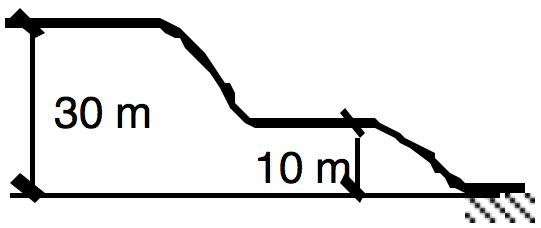
\includegraphics[width=0.95\linewidth]{fnt221-8-hill}
	\vspace{-10pt}
\end{wrapfigure}

\noindent A skier (of mass \unit[55]{kg}) skies down the smooth (frictionless) ski slope illustrated in the cross-sectional diagram. She pushes off at the top with a speed of \unitfrac[10]{m}{s}. At the bottom (\unit[0]{m}), she comes to a stop by digging her skis in sideways.\\

\noindent Use the algebraic expression of energy conservation that shows that the sum of all the energies at all points in time is constant and equal to the total energy for the following:

\begin{enumerate}[(a)]

	\item Pick a location to set $y = 0$ and determine the total energy of the system.
	\item Write an algebraic representation expressing energy conservation that you could use to find the speed of the skier when she is on the middle flat part (at the height \unit[10]{m}).
	\item Substitute all known values of constants and variables, and identify any unknown(s).
	
\end{enumerate}
